\documentclass[11pt]{article}

%% ----------------------------------
%
%     Packages to be used in the final manuscript
%
%% ----------------------------------


%\usepackage[margin=1in]{geometry}

% use proper unicode fonts
\usepackage[T1]{fontenc}
\usepackage[utf8]{inputenc}

\usepackage{amsmath} % for better display of equations

\usepackage{setspace}
\usepackage{natbib} 
 
\usepackage{titling} % controls the way the title information is displayed
\pretitle{\begin{flushleft}\Large}
\posttitle{\end{flushleft}}
\predate{}
\postdate{}
\preauthor{\begin{flushleft}}
\postauthor{\end{flushleft}}
\setlength{\droptitle}{-3em}

\usepackage{authblk} % adds some nice options for displaying the author list
\renewcommand\Authsep{\protect\\}
\renewcommand\Authands{\protect\\}

\usepackage{acronym} % set up some acronyms
\acrodef{SDM}{species distribution model}
\acrodef{MCMC}{Markov Chain Monte Carlo}

%% graphics packages
\usepackage{graphicx}
\usepackage{pdflscape}   % for figures in landscape orientation
\usepackage[labelsep=none]{caption}

% Tikz libraries for building the diagram
\usepackage{tikz}
\usepackage{tikz-cd}
\usetikzlibrary{calc, shapes}
\usetikzlibrary{shapes.geometric,shapes.arrows,decorations.pathmorphing}
\usetikzlibrary{matrix,chains,scopes,positioning,arrows,fit}

\usepackage[pagewise]{lineno}


%% ----------------------------------
%
%     Packages to be used for drafts and editing
%     Remove from the final manuscript
%
%% ----------------------------------
\usepackage[top=1in, left=1in, bottom=1in, right=2.5in]{geometry}

\usepackage[textsize=tiny, backgroundcolor=white, textwidth=2.2in, colorinlistoftodos=true]{todonotes} % for margin notes using \todo{}

%%% available colors:
%%% red, green, blue, cyan, magenta, yellow, gray, drakfray, lightgray, brown, lime, olive, orange, pink, purple, teal, violet
%
%\newcommand{\mt}[1]{\todo[color=blue!40]{\textsuperscript{MT}#1}}
%\newcommand{\ib}[1]{\todo[color=magenta!40]{\textsuperscript{IB}#1}} 				
%\renewcommand{\aa}[1]{\todo[color=violet!40]{\textsuperscript{Aitor A}#1}}
\newcommand{\ia}[1]{\todo[color=blue!20]{\textsuperscript{Isabelle A}#1}}
\newcommand{\db}[1]{\todo[color=violet!20]{\textsuperscript{Dominique B}#1}}
%\newcommand{\ab}[1]{\todo[color=teal!40]{\textsuperscript{Alyssa B}#1}}
%\newcommand{\fd}[1]{\todo[color=orange!30]{\textsuperscript{Frédérik D}#1}}
%\newcommand{\rd}[1]{\todo[color=orange!40]{\textsuperscript{Ronnie D}#1}}
\newcommand{\mjf}[1]{\todo[color=green!60]{\textsuperscript{Marie-Josée F.}#1}}
%\newcommand{\tf}[1]{\todo[color=yellow!60]{\textsuperscript{Tony F.}#1}}
\newcommand{\dm}[1]{\todo[color=lime!50]{\textsuperscript{Dan M.}#1}}
\newcommand{\ks}[1]{\todo[color=green!40]{\textsuperscript{Kevin S}#1}}
%\newcommand{\ns}[1]{\todo[backgroundcolor=red!100, linecolor=orange!100, bordercolor=cyan!100]{{\color{magenta!40}\textsuperscript{Strigul}#1}}}
\newcommand{\wt}[1]{\todo[color=orange!80]{\textsuperscript{Wilfried T}#1}}
\newcommand{\dg}[1]{\todo[color=pink!40]{\textsuperscript{DG}#1}}

% uncomment to disable individual authors
% \renewcommand{\mt}[1]{\relax}%
% \renewcommand{\ib}[1]{\relax}%
% \renewcommand{\aa}[1]{\relax}%
% \renewcommand{\ia}[1]{\relax}%
% \renewcommand{\db}[1]{\relax}%
% \renewcommand{\ab}[1]{\relax}%
% \renewcommand{\fd}[1]{\relax}%
% \renewcommand{\rd}[1]{\relax}%
% \renewcommand{\mjf}[1]{\relax}%
% \renewcommand{\tf}[1]{\relax}%
% \renewcommand{\dm}[1]{\relax}%
% \renewcommand{\ks}[1]{\relax}%
% \renewcommand{\ns}[1]{\relax}%
% \renewcommand{\wt}[1]{\relax}%
% \renewcommand{\dg}[1]{\relax}%

%% ----------------------------------
%
%     Title and authorship information
%
%% ----------------------------------


\title{Cross-scale integration of knowledge for predicting species ranges: a metamodeling framework}
\date{}
\author[1,2,13]{Matthew V. Talluto (mtalluto@gmail.com)}
\author[1,2]{Isabelle Boulangeat (isabelle.boulangeat@gmail.com)}
\author[3]{Aitor Ameztegui (ameztegui@gmail.com)}
\author[4]{Isabelle Aubin (Isabelle.Aubin@NRCan-RNCan.gc.ca)}
\author[1,2,5]{Dominique Berteaux (Dominique\_Berteaux@uqar.ca)}
\author[1,2]{Alyssa Butler (ca.butler10@gmail.com)}
\author[6,7]{Frédérik Doyon (Frederik.Doyon@uqo.ca)}
\author[8]{C. Ronnie Drever (cdrever@TNC.ORG)}
\author[9]{Marie-Josée Fortin (fortinmj@gmail.com)}
\author[1]{Tony Franceschini (Tony.Franceschini@uqar.ca)}
\author[10]{Jean Liénard (jean.lienard@gmail.com)}
\author[4]{Dan McKenney (Dan.McKenney@nrcan-rncan.gc.ca)}
\author[2,3]{Kevin A. Solarik (kevinsolarik@hotmail.com)}
\author[10]{Nickolay Strigul (nick.strigul@vancouver.wsu.edu)}
\author[11, 12]{Wilfried Thuiller (wilfried.thuiller@ujf-grenoble.fr)}
\author[1,2]{Dominique Gravel (dominique\_gravel@uqar.ca)}
\affil[1]{Département de biologie, Université du Québec à Rimouski, Rimouski, Quebec, Canada}
\affil[2]{Quebec Centre for Biodiversity Science, Montreal, Quebec, Canada}
\affil[3]{Centre d'Étude de la Forêt, Département des sciences biologiques, Université du Québec à Montréal, Montreal, Quebec, Canada}
\affil[4]{Great Lakes Forestry Centre, Canadian Forest Service, Natural Resources Canada, Sault Ste Marie, Ontario, Canada}
\affil[5]{Centre for Northern Studies, Université du Québec à Rimouski, Rimouski, Quebec, Canada}
\affil[6]{Université du Québec en Outaouais, Gatineau, Quebec, Canada}
\affil[7]{Institut des Sciences de la Forêt Tempérée (ISFORT), Ripon, Quebec, Canada}
\affil[8]{The Nature Conservancy Canada, Ottawa, Ontario, Canada}
\affil[9]{Department of Ecology and Evolutionary Biology, University of Toronto, Toronto, Ontario, Canada}
\affil[10]{Department of Mathematics, Washington State University Vancouver, Washington, USA}
\affil[11]{Université Grenoble Alpes, Laboratoire d’Ecologie Alpine (LECA), F-38000 Grenoble, France}
\affil[12]{CNRS, Laboratoire d’Ecologie Alpine (LECA), F-38000 Grenoble, France}
\affil[13]{Author for correspondance. Address: Departament de Biologie, chimie, et geographie, 300, Allée des Ursulines, Rimouski, Quebec G5L 3A1, Canada}


%% ----------------------------------
%
%     END PREAMBLE
%
%% ----------------------------------

\begin{document}
\doublespacing
%% ----------------------------------
%
%     TITLE PAGE
%
%% ----------------------------------

%TC:ignore
\begin{titlingpage}
	\maketitle
	
	\begin{flushleft}
	
	% less than 45 chars including spaces
	\textbf{Short title:} Integrated models of species ranges

	\textbf{Type of article:} Ideas and Perspectives
	
	% abstract limited to 200 words
	% main text excludes abstract, acknowledgements, references, table and figure legends; limited to 7500 words
	% boxes limited to 750 words each
	% figure captions limited to 150 words each
	\textbf{Word counts: } Abstract: 200; Main Text: 6086; Boxes: 517

	\textbf{Number of references:} 79 % limited to 80

	\textbf{Number of figures:} 6
	
	\textbf{Number of tables:} 0
	
	\textbf{Number of text boxes:} 1
	
	\textbf{Authorship:} All authors contributed substantially to an initial outline of the paper and ideas. MT, IB, and DG built the model and wrote the first draft of the introduction and model description. All authors contributed to the complete first draft and all subsequent revisions to the manuscript.
		
	\textbf{Keywords:} Climate change, decision making, metamodeling, patterns and processes, range dynamics, scaling, spatial ecology, species distribution modeling, uncertainty
	\end{flushleft}
\end{titlingpage}
%TC:endignore

%TC:break abstract
\linenumbers
\begin{abstract}
\ia{Some section of the manuscript are a bit long and may be shorterned. I have made some suggestion but I think it should be shorten more.}
\ia{The abstract would need a bit of work in the formulation and editing. I have made some suggestions.}
% limited to 200 words
There is great interest in modeling species ranges, resulting in a great diversity of modeling approaches.
\dm{There is great interest in modeling species ranges – both potential and actual, resulting in a great diversity of modeling approaches.}
However, in general, individual approaches include only a small subset of the total available information about a species. 
\ia{delete first two sentences, replace with: \\
Current worldwide preoccupations with species range shifts have resulted in a great diversity of approaches in species range modelling. Each approach typically includes only a small subset of the total available information about a species; correlative models customarily predict...}
Correlative models often predict presence or absence as a function of climate, but ignore  smaller-scale processes such as growth, fecundity, and dispersal.
\ia{see suggestion for a rewrite of the remainder:\\
What’s more, these approaches frequently result in divergent predictions, with no straightforward method to reconcile them. We present a flexible framework allowing the integration of models across multiple scales. Using hierarchical Bayesian methods, we produce ametamodel which, by incorporating all of the information used as input for the original scale-specific sub-models, produce probabilistic estimates of species presence andreports uncertainty from both data and process error. We provide two contrasting examples to illustrate our approach, and demonstrate that it can substantially reduce uncertainty when projecting beyond the range of the original data. Our method could be an invaluable tool for conservation biologists and land managers, despite the technical challenge of its actual implementation. We strongly encourage collaboration between modelers and practitioners in overcoming these hurdles and achieving greater integration of knowledge, a goal which we are confident will be of wide interest.
}
Furthermore, the diversity of approaches often results in divergent predictions for the same species, with no simple way to reconcile these predictions.
We present a flexible framework for integrating models at multiple scales using hierarchical Bayesian methods. 
The resulting metamodel produces probabilistic estimates of species presence, reports uncertainty from both data and process error from all sub-models, and incorporates all of the information used as input for the original scale-specific sub-models.
\ks{Change above to:\\
The resulting metamodel produces probabilistic estimates of species presence, reports uncertainty from both data and process error from all sub-models used, while also  synthesizing all of the information as an input for the original scale-specific sub-models.}
We illustrate our approach using two examples, and demonstrate that the framework can substantially reduce uncertainty when projecting beyond the range of the original data.
We conclude by discussing the application of our method and its accessibility to conservation biologists and land managers.
\dg{That’s the smartest comment of the whole paper!!!}
Although implementation of our method can be technically challenging, we anticipate the results will be of wide interest, and we encourage collaboration between modelers and practitioners in applying our framework.
\end{abstract}

%TC:break manuscript
%% ----------------------------------
%
%     INTRODUCTION
%
%% ----------------------------------

\section*{Introduction}

Models of species range limits have wide applications and can play a large role in conservation biology, where they can be used as decision-making tools in biodiversity management \citep{Guisan2013}.
\ia{This sentence is repetitive and somewhat contradictory with the last one of the paragraph. Suggest deletion}
Due to large temporal and spatial scales as well as the complex and nonlinear nature of ecosystem dynamics, it is often impossible to construct experiments that can adequately explore the ecological processes generating species range limits \citep{Wu1995, Levin1998}. 
Hence, range models are essential tools that have been applied to a large number of ecological subfields, including biogeography \citep{Schurr2012}, invasion biology \citep{Catterall2012, Gallien2012}, evolution \citep{Jay2012}, hybrid zone dynamics \citep{Engler2013}, and forecasting the impacts of climate change on species distributions \citep{Thuiller2011, Blois2013, Thuiller2014}. 
However, despite having recognized potential to support decision making, the contributions of these models to conservation and applied ecology remain limited \citep{Guisan2013}.

\ia{Miss one sentence here. To make a link with the sentence above, you should briefly state why models contribution remains limited. }
Two important constraints on modeling ecological processes can prevent models from making unbiased predictions with acceptable uncertainty: (1) having the appropriate ecological theory needed to link data to modeling objectives, and (2) having sufficient data over a range of conditions to maintain coherence between the spatial and temporal scales of data and theory.
Another constraint is a paucity of data over wide ranges of ecological conditions and scales.
\dg{change to:\\
The paucity of data over theses ecological conditions and scales is a severe constraint. }
Poor data or incoherent models will result in predictions with unacceptably high uncertainty or precise but biased predictions.
In recent decades, however, modeling techniques have proliferated to take advantage of what is available in terms of both data and modeling platforms.
Model diversification also arises due to the diverse processes generating species ranges \citep{Soberon2007}.
\dg{Just to encourage self citation, this paper is more recent and supported by data, not only discussion: \\

 Boulangeat, I., Gravel, D. and Thuiller, W. 2012. Disentangling the underlying mechanisms of species abundance distribution using a comprehensive and nested modeling framework. Ecology Letters 15 : 584-593. }
In the context of forecasting, which is the focus here, mechanistic and correlative approaches represent quite different modes of inference, but both have strong limitations. 
\ia{delete "which is the focus here"}
Fine-scale mechanistic models may capture important ecological processes quite well, but due to their specificity, they may perform poorly when applied at the scale of species ranges.
For instance, biotic interactions (including trophic interactions) are usually not modeled mechanistically at the scale of species distributions because they are poorly known, or have not been recorded, despite being considered a key determinant of range limits \citep{Holt2005, Soberon2007, Pigot2013}. 
On the other hand, coarse-scale correlative models statistically relating species occurrences to associated distributions of other variables have the advantage of indirectly accounting for underlying processes \citep{Guisan2000}.
However, their predictions rely on the constancy of the relationships between occurrences and explanatory variables in time and space, implying that the selected variables are related to the processes limiting species ranges and that their correlations are constant for calibration and projection ranges in space and time \citep{Dormann2007}. 
Extrapolating beyond the scope of the original data (e.g., predicting ranges based on future climate) is therefore problematic, because nonlinearities in responses to novel combinations of the explanatory variables cannot be accommodated in models that do not simulate the underlying processes.
In cases where a selected explanatory variable indirectly accounts for a process (e.g., where the strength of biotic interactions are correlated with an environmental variable), extrapolation will produce biased predictions in temporal and spatial domains where the process and the environmental variable are decoupled.
Furthermore, correlative models often do not explicitly incorporate ecological processes into their formulations, and when applied at coarse scales, they may miss important fine-scale processes, making a multi-scale approach desirable when accurate forecasting is required \citep{Thuiller2013}.
\ia{replace: \\
 desirable when accurate forecasting is required \\
with:
 more suitable}
On the other hand process-based models often require a variety of assumptions which may be poorly understood across space and time.
\ia{Finish abruptely here. Feels like one sentence is missing}
\ks{Feels like it is getting snuck in here…almost an after thought… I would recommend either removing it or developing it a tad further. }
%% ----------------------------------
%% ----------------------------------
%% ----------------------------------

\subsection*{Toward an integrated approach for modeling ranges}
To include knowledge of species from multiple sources and scales into distribution models, we present an application of hierarchical Bayesian methods that uses outputs from multiple model outputs to inform the results of the final model.
Our approach is an alternative to other approaches to multimodel inference that offers improved flexibility in incorporating data and theory from multiple scales and provides transparent estimation of uncertainty.
The challenge is to account for all this available knowledge while producing a single prediction, potentially mitigating the limitations inherent in each modeling approach and contributing to more robust predictions \citep{Pearson2003, Guisan2005, Araujo2006, Quillet2010}.
\ia{replace above sentence with: \\
``By producing a single prediction from multiple models, we aim at mitigating the limitations inherent in each modeling approach and contributing to more robust predictions ''}
\ks{change previous 2 sentences to:\\
Our approach succeeds in providing a much more throrough implementation of data from multiple models, while incorportating multiple scales and transparency in our estimation of uncertainty. A number of challenge(s) arised with this approach: (1) accounting for all the available data, (2) producing a single congruent prediction from all the models implemented, and (3) mitigating the potential limitations within each modeling approach }
Some researchers have explicitly reproduced the hierarchical nature of ecological systems using hierarchical models \citep[e.g.][]{Royale2008, Boulangeat2012, Catterall2012, Strigul2012, Soranno2014}. 
Recent literature has also focused on the development of hybrid models, which allow for flexible combinations between mechanistic and phenomenological sub-models \citep{Gallien2010, Thuiller2013}. 
For instance, correlative models are used to account for abiotic variables limiting species distributions \citep{Guisan2005}, while mechanistic approaches can include space and time dynamics and therefore account for dispersal processes \citep{Kearney2008}. 
This complementarity has been used to merge the two model types into hybrid integrated models \citep[e.g.][]{Keith2008, Anderson2009, Smolik2010, Boulangeat2014}. 
\wt{Dormann et al. suggested to separate hybrid and integrated. 
Dormann, C.F., Schymanski, S.J., Cabral, J.S., Chuine, I., Graham, C.H., Hartig, F., Kearney, M., Morin, X., Römermann, C., Schröder, B. \& Singer, A. (2012) Correlation and process in species distribution models: bridging a dichotomy. Journal of Biogeography,
}
However, the link between different sub-models is based on assumptions about the scaling of ecological processes that are not easy to test \citep{Gallien2010},
\wt{and hardly known}
and uncertainties are very difficult to quantify and identify from its many different sources. 
Moreover, hybrid approaches are not suitable for merging models that are based on the same processes but with different underlying hypotheses.

A second approach is to directly combine predictions.
\ia{A second approach recently explored by modelers is to directly combine predictions.}
If models operate at the same scale and have compatible parameterizations, predictions can be combined using multi-model inference \citep[e.g., model averaging, ensemble forecasting;][]{Thuiller2004, Araujo2007}. 
If models are not comparable because they are based on different data or hypotheses, the use of convergent predictions from multiple models is a way to provide more robust projections \citep{Morin2009, Marmion2009, Serra-Diaz2013}.
\wt{Cheaib, A., Badeau, V., Boe, J., Chuine, I., Delire, C., Dufrêne, E., François, C., Grittid, E.S., Legay, M., Pagé, C., Thuiller, W., Viovy, N. \& Leadley, P. (2012) Climate change impacts on tree ranges: model inter-comparison facilitates understanding and quantification of uncertainty. Ecology Letters, 15, 533-544.}
However, the applicability of ensemble forecasts is limited; for example, it is not currently possible to evaluate the effects of convergent predictions on the total uncertainty of the outcomes.
\ia{paragraph break here}
One of the greatest challenges inherent in both approaches is estimating uncertainty, which is of utmost importance in a prediction context.
A more comprehensive understanding of uncertainty can guide biodiversity management and prioritize future data collection by identifying parameters that make large contributions to the total uncertainty in the model predictions \citep{McMahon2011}. 
In models that encompass multiple scales or levels of organization, it is particularly challenging to evaluate all sources of uncertainty, especially those related to model specification (\citealt{Calder2003} but see \citealt{Conlisk2013}).
\dg{‘uncertainty’ is used 6 times over 5 sentences. Would help some rewording to limit redundancy}
Clearly, an approach that integrates predictions and uncertainty from multiple model types is needed \citep{Beck2012, Thuiller2013}. 
Such an approach would incorporate multiple modes of inference and integrate data from multiple sources and scales \citep{Levin1992, Peters2004, Thuiller2013}.

Here, we present a framework for modeling species range dynamics that aims to account for all the information available on a focal species, from a variety of sources and scales.
Contrary to hybrid and hierarchical models, the aim is not to link different sub-models into a single model, but to condition the predictions of a metamodel at the target scale (e.g., an entire species' range) with information from independent sub-models at a variety of spatial scales, allowing for as much flexibility as possible regarding the type of information included. 
We use the power and generality of a hierarchical Bayesian framework, which allows us to include multiple data sources and modes of inference \citep{VanOijen2005, Clark2006, Hobbs2011, Hartig2012}. 
Another advantage of Bayesian methods is that uncertainty in model outputs is intuitive to interpret and reflects uncertainty at all levels of organization \citep{Cressie2009, Hobbs2011}. 
We illustrate our approach with two examples.
First, we use simulated data to present a complete example of the application of the framework to multiple information sources that are relevant at very different scales.
In a second example, we apply the framework to combine predictions of a correlative model relating the range of sugar maple (\emph{Acer saccharum}), a widespread foundation tree species from eastern North America, to climate with the predictions of a phenological model, Phenofit, with the goal of improving uncertainty estimation when projecting model predictions to future climate.
\dg{ref missing for phenofit}

%% ----------------------------------
%
%     MODELING FRAMEWORK
%
%% ----------------------------------

\section*{Integrated modeling framework}

The key idea of our approach is to constrain the parameters of a correlative metamodel using predictions made by one or several mechanistic sub-models from other spatial scales.
\wt{does not really have to, right? (wrt different scales)}
The role of the metamodel is to integrate data at the same ecological scale as predictions. 
As an example, the metamodel could take the form of a simple correlative \ac{SDM}.
Ideally, each sub-model incorporates different data types and hypotheses that specify underlying ecological mechanisms contributing to the model output.
The output of sub-models should provide additional predictions at a comparable ecological scale at which the metamodel operates, although it is not necessary for the sub-models to actually operate at the same scale.
For sub-models operating at a substantially different scale than the metamodel, scaling functions will be required; however, these functions can be simple while still contributing useful information to the metamodel (see Example 1). 
All predictions may therefore be integrated in a single Bayesian framework when evaluating the parameters of the metamodel (see Box 1, Fig. \ref{fig:diagram}).
We present and apply the framework here with two examples, and follow with a more formal presentation in Box 1.


%% ----------------------------------
%
%     EXAMPLE 1
%
%% ----------------------------------
\subsection*{Example 1: Adding experimental evidence for the fundamental niche to a species distribution model}
\ia{To keep the ms short, the 2 examples can be summarized a bit more and the details put in the Appendix}

In this hypothetical example, we build a metamodel relating the distribution (i.e. occurrence probability) of an annual plant to coarse-scale climate with complementary information originating from a fine-scale experiment manipulating the precipitation regime.
The metamodel attempts to capture the realized distribution of a species; as a correlative model, it implicitly captures the major physiological constraints and ecological processes constraining the distribution of the target species. 
However, for the purposes of forecasting, we would like to disentangle the fundamental response of a species to environmental variation from other processes in order to map the climatic envelope of where a species may be found in a natural setting. 
Prior information of the physiological constraints affecting species distribution is sometimes available, but usually too incomplete to perform a reasonable comparison with the realized distribution.
For instance, as in this example, a species distribution might be constrained by both temperature and precipitation, but experiments were conducted only over a precipitation gradient at one temperature. 
We apply our framework here to such heterogeneous sources of information to reduce the bias in parameter estimation and more adequately represent uncertainty (see Appendix S1 in Supporting Information for procedural details and scripts for executing the model).

We consider data collected from a species' historical distribution, where the goal is to predict the distribution following a substantial reduction in precipitation. 
We will consider \(X_M\) (see Box 1, Fig. \ref{fig:diagram}) to be a vector of $n$ observations that takes the value of one to indicate presence and zero for absence:
\begin{equation}
X_M = \{x_{M,1}, x_{M,2}, \ldots, x_{M,n}\}
\end{equation}
We assume the data are relatively high-quality, providing coverage over a wide region and covering various climatic conditions (Fig. \ref{fig:ex1_sampling}a). 
The model is evaluated by relating these observations to environmental data \((D_M)\), which, for the sake of the example, consists of mean annual temperature $T_M$ and annual precipitation $P_M$. 
For simplicity, we formulate the metamodel \((\theta_M)\) as a simple logistic regression with a second order effect of temperature and precipitation. 
This naive model (i.e., the metamodel with no constraints from sub-models) predicts  occurrence probability (\(\psi_N\)) as a function of the environment:
%-----
\begin{equation}
\begin{aligned}
	\psi_N &= f\left(\theta_M, D_M \right) \\
	&= p \left (X_M = 1 \mid \theta_M, T_M, P_M \right) \\
	&=\text{logit}^{-1}\left( \mathbf{\Theta_M} \mathbf{D_M} \right)
\end{aligned}
\end{equation}
%-----
where \(\mathbf{\Theta_M}\) is the parameter vector of the model \(\theta_M\), \(\mathbf{D_M} \) is the covariate matrix (i.e., \(T_M, P_M\), with the first column taken to be unity to allow an intercept to be fit), and \(\text{logit}^{-1}\) is the inverse of the logit function.
We can fit this model in a Bayesian framework to allow for easy integration of models (as we will show later).
In this context, the goal of modeling is to estimate the probability distribution of \(\theta_M\), the model parameters, given the observed data \((X_M, T_M, P_M)\), which is given by the proportional form of Bayes's Theorem \citep[for readers unfamiliar with general concepts in Bayesian inference, a concise introduction can be found in ][]{Link2010}:
%-----
\begin{equation}
\label{eq:ex1_bayes}
	p\left (\theta_M \mid X_M,T_M,P_M \right ) \propto 
	p \left(X_M \mid \theta_M, T_M, P_M \right)
	p \left(\theta_M \right)
\end{equation}
%-----
where \(p\left(X_M \mid \theta_M, T_M, P_M \right)\) is often referred to as the \emph{likelihood} of the data (\(X_M\)) given the model (\(\theta_M\)), 
\wt{model parameters?}
\(p\left(\theta_M \right)\) is often referred to as the \emph{prior distribution} of \(\theta_M\), and the goal of modeling is to estimate \(p\left (\theta_M \mid X_M,T_M,P_M \right )\), the \emph{posterior distribution} of \(\theta_M\), which gives the probability that \(\theta_M\) takes particular values, given the observed data.

Thus far, we have considered only a single source of information to fit this model, and therefore the prior distribution \(p\left(\theta_M \right)\) from Eq. \ref{eq:ex1_bayes} is uninformative.
As a secondary source of information, we will consider an experiment relating the population growth rate of the plant to manipulations to the precipitation regime, with results (but no raw data) available from the literature (Fig. \ref{fig:ex1_sampling}b). 
Furthermore, no information is available regarding the temperature regime for the experiment.
Transplant experiments that evaluate performance beyond the range of a species are common, and represent a plausible scenario for model integration \citep{Hargreaves2014}.
According to niche theory \citep{Holt2009}, the fundamental niche corresponds to the set of environmental conditions where the per capita intrinsic growth rate $r$ is positive.
This concept gives us a reasonable model to fit the scaling function $g$ for our sub-model (Fig. \ref{fig:diagram}).
If we hypothesize that the errors from Figure \ref{fig:ex1_sampling}b \( \left(\sigma_{S} \right) \) are normally distributed, then for observation $i$, we can interpret the probability of presence \( \left(\psi_{S,i}\right)\) as the probability that the observed growth rate \(X_{S,i}\) is positive:
\begin{equation}
	\psi_{S,i} = \int_0^\infty N \left(X_{S,i}, \sigma_{S,i} \right)
\end{equation}
where \(N\) is the Normal density function.
We can then estimate the posterior distribution for the sub-model by fitting the relationship between \(\psi_S\) and precipitation \( \left( P_S \right) \) using Bayesian beta regression \citep{Ferrari2004}:
%-----
\begin{equation}
\label{eq:ex1_thetas}
	p\left (\theta_S \mid \psi_S,P_S \right ) \propto 
	p \left(\psi_S \mid \theta_S, P_S \right)
	p \left(\theta_S \right) \\
\end{equation}
%-----

Although the two datasets were collected at considerably different scales, we now have sub-model predictions arising from a fine-scale experiment that are relevant at the scale of the metamodel (i.e., the probability of presence at a given precipitation). 
This scaling is quite simplistic, and would never be used to predict a species' range using this mechanistic sub-model in isolation.
Despite the strong theoretical foundation (i.e., niche theory) linking the observations to presence-absence at large scales, the upscaled sub-model (i.e., the transformation of \(X_S\) and \(\sigma_S\) to \(\psi_S\)) is built on the strong hypothesis that the species will be present when $r>0$, neglecting other population dynamics constraints such as Allee effects and metapopulation dynamics. 
The fundamental niche is also incomplete, as we lack environmental variables such as temperature, as well as all other ecological processes responsible for the realized distribution.
As such, it would be unwise to expect predictions from this model alone to resemble the actual distribution of the species; as a mechanistic model, it is simply too incomplete to predict distribution.
As we will show, however, the information from this sub-model, when applied as a constraint on the metamodel, can result in improved predictions that incorporate the information within each model.

We accomplish model integration by treating the posterior of \(\theta_S\) as prior information about some of the parameters of \(\theta_M\) (i.e., parameters related to precipitation), expanding Equation \ref{eq:ex1_bayes} to incorporate the new information from the sub-model:
%-----
\begin{equation}
	\label{eq:ex1_integrated}
	\overbrace{p(\theta_M \mid X_M, T_M, P_M, \theta_S, \psi_S, P_S)}^\text{integrated posterior}
	\propto
	\overbrace{p\left (\psi_S \mid \theta_S,P_S \right )}^{\substack{\text{new information} \\ \text{from sub-model}}}
	\overbrace{p \left(X_M \mid \theta_M, T_M, P_M \right) P \left(\theta_M \right)}^{\substack{\text{naive metamodel} \\ \text{posterior}}}
	\overbrace{p \left(\theta_S \right)}^{\substack{\text{prior for} \\ \text{sub-model}}}	
\end{equation}
%-----
As before, the metamodel \(\theta_M\) can be used to predict the species distribution \((\psi_I)\).
However, these predictions will not reflect only the presence-absence samples in \(X_M\), but will also reflect the information from \(\theta_S\), including all of the data sources used to produce this sub-model.
In other words, with this evaluation, the set of parameters $\theta_M$ is most likely when it agrees with both the original data and predictions from the sub-model. 
Note that in this particular example, because the sub-model is only contingent on precipitation, there is no integration on temperature. 
Finally, we note the presence of marginal distributions for both models (i.e., \(p(\theta_M)\) and \(p(\theta_S)\)).
These can be informative (e.g., incorporating further prior information or the predictions of additional sub-models), semi-informative (e.g., to provide greater weight to more informative models), or uninformative.
For purposes of this example, we used these terms to reduce the precision of the second model to reflect the uncertainty of the modeling process (due to the lack of additional mechanisms in the second model, as mentioned above).

We performed this procedure with our hypothetical datasets.
When comparing the three models (naive metamodel, mechanistic sub-model, and integrated metamodel), we observed extreme uncertainty in the first model when projecting beyond the range of the original data.
\ks{add ref to figure}
Unsurprisingly given the quality of the data, the sub-model was highly precise with respect to precipitation and not useful for temperature, thus providing a fairly strong constraint when producing the integrated model.
The result was an integrated prediction that reflected the shapes of both models and showed considerably reduced uncertainty (Fig. \ref{fig:ex1_precip}).
At the scale of the metamodel, considering both temperature and precipitation, we observed similar results, with reduced uncertainty in the predictions over the domain not covered by the presence-absence data (Fig. \ref{fig:ex1_map}).

Once the technical challenges of evaluating the parameters are overcome, integration has several advantages over both the naive parameterization of the metamodel and the mechanistic sub-model. 
In the situation where both models strongly agree on the relationship between water availability and occurrence probability, then we should expect significantly reduced uncertainty in that domain (Figs. \ref{fig:ex1_precip}, \ref{fig:ex1_map}).
Because the metamodel includes both temperature and precipitation, any reduction in the uncertainty with respect to precipitation might also influence the evaluation of the relationship with temperature (reducing bias in the case where there is a correlation between T and P in the data). 
However, uncertainty could increase in the case of model disagreement.
For instance, the relationship between precipitation and presence in the naive metamodel could be caused by a spurious relationship (e.g. spatial autocorrelation caused by historical contingencies), leading to a false confidence in the species distribution over precipitation gradients. 
The information from the sub-model will thus bring back the right amount of uncertainty in the relationship.
Moreover, convergence in model predictions in overlapping domains (e.g., near the peak in the probability of presence in Fig. \ref{fig:ex1_precip}) can aid in detecting crucial ecological processes.



%% ----------------------------------
%
%     EXAMPLE 2
%
%% ----------------------------------


\subsection*{Example 2: Constraining an SDM using phenological information}
For the second example, we consider the problem of predicting the future distribution 
\wt{forecasting the potential distribution of a species}
of a species following climate change.
There is considerable interest in comparing correlative and mechanistic projections with respect to climate change \citep{Morin2009}, and correctly characterizing uncertainty is a critical aspect of this problem \citep{Cheaib2012}.
Despite being a relatively common application of \ac{SDM}s \citep{Guisan2005}, projecting models parameterized with modern climate data to future climate scenarios remains problematic \citep{Araujo2006}.
We used our metamodeling framework to inform a climate-based SDM with information obtained from Phenofit, a mechanistic model that predicts a species' probability of presence as a function of the suitability of the environment given the species' phenology \citep{Chuine2001, Morin2009}.
We use data from \citet{Morin2009} for sugar maple (\emph{Acer saccharum}), an economically and ecologically important species occurring in eastern North America.
Here we describe briefly the dataset, methods, and the results of the analysis (see Appendix S2 for data and scripts to reproduce the analysis).

\defcitealias{IPCC2001}{IPCC, 2001} % this is needed to make the organizational citation in the following paragraph work correctly
For the metamodel, we used a dataset of 1013 presence and 13863 absence records, at 0.5 degree resolution, sampled from North America.
We reserved one-third of the dataset for validation, and used the area under the receiver operating characters curve (AUC) for validation of contemporary predictions.
We used a binomial GLM to relate the suitability for sugar maple to 6 climate variables, scaled to the same resolution (see Appendix S2 for details on the climate variables).
We selected a GLM here for its simplicity and interpretability because our focus was on demonstrating the framework, but more complex methods (e.g., GAM) are compatible with the framework.
For projection, we used predictions for 2080 from the HadCM3 GCM \citep{Pope2000} driven by the A2 emission scenario \citep{Nakicenovic2000}, and used the parameters of the GLM to forecast suitability into the future (i.e., \(\psi_N\)).
Phenofit produces predictions at continental scales; thus the scaling function \(g\) was incorporated within Phenofit itself and we performed model integration directly on the outputs.
To perform the integration, we used \ac{MCMC} to condition the parameters of the metamodel  on two likelihood functions.
The first is the naive SDM, where the likelihood of a ``success'' in the presence/absence dataset was a Bernoulli density with the (logit-transformed) probability expressed as a linear function of the climate predictors.
For the sub-model, we considered that Phenofit, being a process-based model, may perform better when projecting into the future.
Thus, we used the predicted future probability of presence as the basis for generating simulated future presence-absence datasets.
This procedure inherently incorporates some uncertainty by randomly determining where the species is present (though uncertainty in the probabilities themselves could not be incorporated, as they were not available).
Thus, the sub-model likelihood is simply the probability, given the predictions of the metamodel, of observing a simulated dataset \(X_s\) that is randomly drawn from the phenofit predictions \(\psi_s\); i.e., \(X_s = f(\psi_s)\):
\begin{equation}
\label{eq:integrated2}
	p( \theta_M \mid X_M, D_M, \psi_s, \theta_S )
	\propto 
	p( X_S = f(\psi_s)\mid \theta_M, \theta_S )
	p( Y_M \mid \theta_M, D_M ) 
	p( \theta_M )
	p( \theta_S )
\end{equation}
where \(\theta_M\) is the metamodel, 
\(X_M\) is the vector of contemporary presences and absences, 
\(D_M\) is the matrix of climate predictors,
and \(\theta_S\) is the model relating the Phenofit predictions to the metamodel.
Furthermore, the integration is performed on the \emph{predictions} of the sub-model directly, rather than on compatible parameters as in Example 1. 
Thus, the metamodel must appear in the sub-model likelihood.

For present climates, the predictions of Phenofit (Fig \ref{fig:ex2}A) were largely similar to those of the naive SDM (Fig \ref{fig:ex2}C). 
Furthermore, variance in the predictions of the naive model was relatively low throughout the spatial domain (Fig \ref{fig:ex2}E).
\ks{provide specific figures for variance of the different models}
Similar patterns were repeated for analogous climates under the future scenario (Fig \ref{fig:ex2}D); however these predictions differed considerably from the predictions of the mechanistic sub-model (Fig \ref{fig:ex2}B), and uncertainty for the projection was relatively high, particularly for eastern Canada (Fig \ref{fig:ex2}F).
In general, Phenofit predicted considerably less northward migration by 2080.
The integrated model, which included both the presence-absence data as well as the Phenofit predictions for the future, made intermediate predictions in terms of northward range shifts for sugar maple (Fig \ref{fig:ex2}H).
Globally, the integrated model expressed somewhat more uncertainty 
\wt{for the future}
than the naive model (Fig \ref{fig:ex2}J), reflecting the divergent predictions of Phenofit and the naive model.
\wt{Are you sure? From the map, I would have said the reverse.}
However, in areas where the naive model performed worst (e.g., eastern Canada), the level of uncertainty in the integrated model was similar to the uncertainty in other locations.
Unsurprisingly, integration resulted in worse predictions for the present distribution of the species (Fig \ref{fig:ex2}G) compared with either the naive model or Phenofit in isolation.
Conventional SDMs are quite good at producing empirical models of species distributions under present climatic regimes, and the naive model here could be further improved with the addition of more parameters or the inclusion of ensemble forecasting.
This is due to the integration focusing on future predictions; if integration was desired for the present range of the species (perhaps as a way to more accurately quantify uncertainty), a better approach would have been to use the present predictions from Phenofit.
Unfortunately, validation is difficult for projections, as we lack data to evaluate model performance.
For the desired outcome of this model (future projections), validations against present data may not be useful; the predictions of naive model were superior (AUC = 0.99) to those of the integrated model (AUC = 0.96), yet the future predictions of the integrated model may be more realistic than those of the naive model.



%% ----------------------------------
%
%     DISCUSSION
%
%% ----------------------------------



\section*{Discussion}

\subsection*{Comparison with other methods}
The methods provided here expand upon the motivation of hybrid models to develop a more robust and unifying approach for ecological models in a predictive context while striving to overcome some of the limitations characteristic of other integrated approaches. 
Attempting to incorporate underlying ecological processes so that SDMs are not oversimplified by combining different model parameters or scales can be challenging using hybrid approaches. 
In particular, it can often be difficult to identify parameters that can be used to connect different modeling frameworks and which parameters can produce meaningful responses \citep{Thuiller2013}. 
The methods presented in this study aim to overcome some of these limitations through the use of Bayesian statistics. 
Bayesian methods produce results as an entire distribution instead of a single point, allowing for a comprehensive understanding of the uncertainty of estimates \citep{Link2010}. 
The estimation of model parameters (and predictions) as distributions can also help decrease overparameterization that can be a concern for hybrid models. 
Bayesian methods also provide a natural framework for the incorporation of multiple sources of information. 
The inability or difficulty to include information from experimental studies or ecological processes at lower scales can be a possible drawback of hybrid models \citep{Thuiller2008, Smolik2010}. 
\wt{Thuiller, W., Münkemüller, T., Schiffers, K.H., Georges, D., Dullinger, S., Eckhart, V.M., Edwards, T.C., Gravel, D., Kunstler, G., Merow, C., Moore, K., Piedallu, C., Vissault, S., Zimmermann, N.E., Zurell, D. \& Schurr, F.M. (2014) Does probability of occurrence relate to population dynamics?  Ecography,}
Even when a link can be formed to include this information, it often is oversimplified to facilitate computation \citep{Gallien2010}. 
Finally, Bayesian methods inherently allow for feedbacks or interactions between sub models, which may be a more realistic representation of ecological dynamics where many factors may simultaneously influence the system.

Our approach is an original application of Bayesian multilevel modeling, and can be considered a logical extension of other Bayesian approaches developed to deal with processes that occur at multiple scales while using several models simultaneously. 
In particular, this development has certain similarities with Bayesian model averaging, Bayesian calibration of process-based models, and hierarchical Bayesian modeling. 
Bayesian model averaging aims to combine several alternative models to obtain better predictions while taking into account parameter uncertainties \citep{Hoeting1999}, and has been applied numerous times in ecology where the mechanisms underlying a complex phenomenon are often unknown \citep[e.g.,][]{Wintle2003, Link2006}. 
Bayesian model averaging considers models operating at the same scale and the posterior distribution is usually determined with Gibbs sampling. 
Bayesian calibration of process-based model focuses on uncertainty of the parameter values, in this case the values of the parameters are calibrated by the model output \citep{VanOijen2005, Hartig2012}. 
In contrast with Bayesian model averaging and calibration techniques, our approach handles data and models operating at different hierarchical scales, and uses process-based models to constrain the shape of a generally more correlative metamodel.
Similar hierarchical approaches have been applied to diverse fields, including engineering \citep{Booth2013}, hydraulic conductivity models \citep{Dostert2009, Efendiev2005}, and climate and atmospheric modeling \citep{Mcmillan2010, Kang2012}.
Although our method as presented is distinct from Bayesian model averaging, it is fully compatible with these methods.
Multiple metamodels could be averaged in this way if a consensus prediction from multiple metamodels (containing, e.g., different sub-model sets or different metamodel formulations).
Furthermore, the metamodel can easily be incorporated into a broader multimodel inference scheme.
For example, the metamodel can be used as one input in an ensemble forecasting scheme that also incorporates other common SDM formulations (e.g., Random Forest, MaxEnt).
\wt{That would be  a bit weird, is not it? I do not see the point of incapsulating the metamodel into a more basic model. I would actually drop that last sentence}

%\fd{FD will work on this part: \\
%It would be good to compare this approach with the kind of one develop by Moorcroft et al. 2001 : Moorcroft, P. R., Hurtt, G. C., \& Pacala, S. W. (2001). A method for scaling vegetation dynamics: the ecosystem demography model (ED). Ecological monographs, 71(4), 557-586.\\
%%Medvigy, D., Wofsy, S. C., Munger, J. W., Hollinger, D. Y., \& Moorcroft, P. R. (2009). Mechanistic scaling of ecosystem function and dynamics in space and time: Ecosystem Demography model version 2. Journal of Geophysical Research: Biogeosciences (2005–2012), 114(G1).\\
%Fisher, R., McDowell, N., Purves, D., Moorcroft, P., Sitch, S., Cox, P., \& Ian Woodward, F. (2010). Assessing uncertainties in a second-generation dynamic vegetation model caused by ecological scale limitations. New Phytologist, 187(3), 666-681. 
%\\
%These models are multilevel and use scaling functions using statisitical moments series.
%}

%----------------------------
%----------------------------
%----------------------------

\subsection*{Advantages of Model Integration}
Species distribution models are important tools that are increasingly used by land managers to face challenges associated to decision-making \citep{Guisan2013}.
A growing number of approaches are available, but they can provide diverging answers to very similar questions due to the differences in their assumptions and methodology. 
This can create confusion and even some mistrust towards models, and some managers may be discouraged from incorporating model results in their management plans. 
Integrated approaches have gained momentum in recent years, with integrative science being featured as a central theme for several science-based governmental organizations around the world \citep[e.g.,][]{Bernier2013}. 
Incorporating information from multiple sources, particularly with respect to uncertainty,  fosters a connection between scientifically-generated knowledge and policy, and is therefore an important tool for adaptive management \citep[][Fig. \ref{fig:management}]{Rehme2011}.
Such approaches are needed in formulating management plans for vulnerable species and ecosystems to avoid basing decisions on too-narrow subsets of the available information \citep{Dawson2011}.
The flexibility of our approach may also represent an advantage for management by easing the integration of specific decision making criteria (e.g. desired grain and extent of outputs) into model development. 
Successful use of an integrated modeling approach will always remain dependent on an intimate understanding of the decision-making process by modelers, emphasizing the importance of close collaboration between with practitioners at all stages of model development \citep{Guisan2013}.
\dm{add\\
Notably the connection between modelers and decision-makers who would use these types of modelsis also critical and the complexities of this relationship should not be trivialized.}

Model uncertainty is another key factor affecting applicability of model outputs \citep{Addison2013}.
One of the main strengths of our approach is that it allows for a clear, transparent identification of uncertainties and how they are transmitted throughout the modeling process. 
Transparency in uncertainty can be considered as a sort of sensitivity analysis, in which areas with large uncertainty can be detected and new experimental research or additional data collection can be designed accordingly (e.g., Example 1, Figs. \ref{fig:ex1_sampling}, \ref{fig:ex1_precip}).
The new knowledge resulting from this research can be readily incorporated into the metamodel, allowing for an iterative learning process that will undoubtedly contribute to reduce uncertainty in predictions for a wide range of environmental conditions. 
Moreover, our framework embraces change as a fundamental process and is able to adapt and respond to it. 
The ease of incorporating new knowledge to the modeling framework (including new theory or the result of management and experimental efforts) will allow for a rapid adjustment of the predictions and the incorporation of the most recent available knowledge into management plans \citep{Keith2011}, and the integration of sub-models allows for clear specification of desired model outputs (via the specification of the metamodel) while easily retaining important ecological objectives (via careful specification of sub-models).
Transparency in the model building process must be accompanied by a clearly documented modeling workflow; the transparency of our approach (and the utility of specifying specific objectives accompanied by appropriate sub-models) will assist in the development of transparent and well documented workflows describing the process of model integration and will ensure reproducibility and applicability (Fig. \ref{fig:management}). 
In an era of continuous and unprecedented change, adaptive approaches such as the one presented here are often highlighted as a pressing need in order to develop strategies to promote ecosystems that are both feasible and resilient \citep{Seastedt2008, Mori2013}.

In many cases, both the data and theory needed to apply our method already exist, and all that is needed is the development of sub-models and the links between the sub-models and a metamodel.
For example, climatic gradients may mediate competitive interactions \citep{Kunstler2011}, which means that simple correlative models that fail to account for competition may be wrong if the climate-competition association changes in the future.
In North America, the US Forest Service maintains a long term Forest Inventory Analysis database that could be utilized to parameterize a competition model.
Such a model need not explicitly predict occurrence limits; rather it could be integrated with a larger-scale model to include information about competition in a distribution model.
The phenological information needed to parameterize the sub-model for Example 2 is similarly available for a wide range of species \citep{Morin2009}.
There are also a number of networks collecting high-quality data with good temporal and spatial coverage (e.g., the National Ecological Observatory Network; NEON, and Long-Term Ecological Research sites; LTER).
There is great potential for these kinds of data to be used in fitting sub-models of the kind used in Example 1.
In other cases, qualitative model comparison efforts have already been made \citep{Morin2009, Cheaib2012}.
Our framework could be used \emph{post-hoc} on the outputs of these models to quantify uncertainty resulting from model disagreement.

%----------------------------
%----------------------------
%----------------------------

\subsection*{Challenges} 
Although our approach is highly flexible and can be applied in a number of situations, there are some challenges to successfully using the framework.
As with any modeling effort, good model specification with strong links to theory are essential \citep{Austin2007}.
Poorly specified models will produce outputs that are uninformative or misleading, and model integration is not a cure for these problems.
In the worst case, constraining a metamodel with a poor sub-model can result in outcomes that are worse in terms of bias and uncertainty than those produced by a naive model.
We expect model selection will play an important role in applications of our framework, and such schemes can be incorporated relatively easily \citep{Madigan1995, Wasserman2000, Tenan2014}.

\dg{but we should also see our approach as a mean to circumvent cases where this happens, since additional information will still be better than anything else}
In a similar fashion, the quality and availability of data impose a significant constraint on the number and type of models that can be implemented.
The capacity to implement a model is very low if data requirements are prohibitive. 
Adequate and unbiased coverage of explanatory variables is a significant obstacle, and exploratory analyses can be a significant aid in understanding how data coverage impacts resulting predictions \citep{Mckenney2002}.
Integration can ameliorate these issues to some extent by using supplemental information (and conceptual advances) in additional sub-models where coverage is weak (e.g., Example 1, Figs. \ref{fig:ex1_precip}, \ref{fig:ex1_map}).
For example, \citet{Freckleton2009} estimated that data are too limited to successfully develop highly mechanistic models predicting weed population numbers. 
A strong asset of our approach is that it can be used without the full suite of data that would be required to run a fully mechanistic model. 
Given that the metamodel is correlative, it can be effectively implemented with, e.g., only presence-absence data, or, in the case where true absences are difficult to obtain, with presences and pseudo absences (provided sufficient care is used in interpreting the results of such a model).
Then any additional mechanistic data that are available will enhance predictions by constraining outputs of the metamodel. 

Finally, determining the functions to use to express the likelihood of the sub-models given the metamodel (i.e., Eqs. \ref{eq:ex1_integrated}, \ref{eq:integrated2}) is a critical point.
In the context of integrated models, the challenge is three fold: (i) which spatial and temporal scales (i.e. which processes), are to be considered, (ii) how to build a scaling function that is consistent with the metamodel and (iii) how error and uncertainty propagate from the sub-models to the metamodel. 
Although we argue that our proposed framework is able to easily deal with very different scales and that the Bayesian framework allows for an efficient integration of uncertainty throughout all scales considered, the building of scaling functions deserves further investigation. 
We have shown in our examples that even simple scaling functions can provide reasonable constraints on the metamodel. 
However, it is likely that the modeling process may include multiple scaling functions operating at different scales when taking all known processes and models into account. 
Indeed, if species distributions are a function of, e.g. poopulation growth rate \citep{Sykes1996, Guisan2000}, they will involve processes at the individual (e.g. competition) or cellular (e.g. photosynthesis) scales. 
Such very large differences in spatial scales imply that simple functions will be inadequate, requiring more traditional upscaling methods. 
Therefore, intermediate models and processes will need to be introduced, and this will require additional parameters, assumptions, and data, and will add uncertainty to the final integrated model.

In an applied context, the results of models predicting species ranges are increasingly used by resource managers, conservation biologists, and forest ecologists for formulating and adjusting recommendations. 
The utility of such models depends on their ability to help evaluate events beyond the bounds of the available data, including in future situations constrained by climate change. 
Practitioners may judge model usefulness on two criteria: (1) Does the model provide reliable predictions at the needed time and space scales, and (2) can the model be implemented given the available data and technical expertise? 
Since most decision makers work at local space scales and follow specific time frames, modelers face the obvious challenge of providing detailed outputs while facilitating implementation.
In terms of model outputs, our framework is transparent in terms of uncertainty by virtue of providing easily interpretable probability distributions for model parameters and predictions.
However, developing the models requires careful model specification, understanding of applied Bayesian methods, and, in some cases, extensive programming.
In many cases, off-the-shelf software can adequately express the model likelihoods with minimal programming, but more complicated models will require the development of custom software.
Thus, this framework will require significant investment in developing customized code for the samplers in order to actually estimate parameters, which may be technically challenging for some practitioners and may limit the adoption of these methods by both practitioners and decision-makers.
However, the same was true of all statistical techniques or modeling approaches when they were initially developed, and many of the conceptual challenges associated with Bayesian statistics are being reduced as they gain recognition in the scientific literature. 
We therefore argue that our proposed approach has a strong potential for direct use in our real world where climate is quickly changing and conservation practices must be adjusted accordingly.
We further argue that forging stronger collaborations between modelers, decision-makers, and practitioners will improve the incorporation of this and other new methods into applied ecology and conservation.


%----------------------------
%----------------------------
%----------------------------

\subsection*{Future directions}
Hierarchical Bayesian modeling requires data at every scale to fit the parameters required to constrain one level with another.
Moreover, beyond the needs for additional data, more knowledge of the important processes driving species range limits is needed to allow for extrapolation beyond the scope of the original datasets to address future changes due to climate and land-use changes.
This knowledge can be obtained through a series of experimental manipulations and by substituting space for time data along environmental gradients.
When experiments are possible, gaps in knowledge can be inferred using surrogate variables, theoretical models and spatially explicit models to explore the range of outcomes possible \citep{Fortin2012}. 
Another way to gain knowledge is to simplify species complexity into a series of states and to use state-transition models (e.g., Markov chain, semi-Markov chain, matrix projection model, integral projection model) which require more theoretical or coarser knowledge of species responses to biotic and abiotic changes.
Although fewer states allow us to better capture the essence of species responses to environmental conditions, knowledge is still required to model feedback effects across processes and spatio-temporal scales.
Hence we need to determine which processes are the most important at a given scale and how to weight their effects while scaling-up.
Our metamodeling approach can act as a springboard for incorporating imperfect knowledge of how multi-scale processes influence species ranges.
By incorporating this knowledge into species distribution models, we can hopefully both reduce bias and more accurately assess model uncertainty when forecasting future changes to species ranges.
%---------------------------------------------
%---------------------------------------------

%TC:ignore
\nolinenumbers
\section*{Acknowledgements}
We acknowledge funding from the Quebec Centre for Biodiversity Science as well as NSERC strategic grant 430393-12. Comments from Charles Canham and William Godsoe improved a previous version of this manuscript. WT received support funding from the European Research Council under the European Community's Seven Framework Programme FP7/2007-2013 Grant Agreement no. 281422 (TEEMBIO). 
%TC:endignore


%TC:break references
%% ----------------------------------
%
%     REFERENCES
%
%% ----------------------------------

\renewcommand\refname{Literature Cited}
\bibliography{model_integration}{}
\bibliographystyle{model_integration}



%% ----------------------------------
%
%     FIGURES
%
%% ----------------------------------

\newpage
\section*{Figure Captions}


\begin{flushleft}

%==================
% FIGURE 1
%% 149 words
%TC:break fig 1
\textbf{Figure \ref{fig:diagram}:}
	The parameters of a correlative metamodel model (left column) are conditioned on the predictions of a mechanistic sub-model (right column).
	The metamodel ($\theta_M$) operates at a single scale and uses occurrence data (\(X_M\)) and explanatory variables ($D_M$) to produce a naive (i.e., not conditioned on sub-models) prediction $\psi_N$.
	The mechanistic sub-model \(\theta_S\) includes data about the response (\(X_S\)) of lower-level behaviours of the system to explanatory variables ($D_S$). 
	The models are integrated by calibrating $\theta_M$ to data ($X_M, D_M$) as well as the output of the sub-model ($\psi_S$). 
	This is possible because predictions from the sub-model ($\psi_S$) emerge at the scale of the metamodel via a scaling function \(g(\theta_S, D_S)\).
	This prediction incorporates multiple sources of information coming from several calibration datasets (i.e., $X_M, D_M, X_S, $ and $D_S$) as well as from multiple types of models (i.e., $\theta_M$ and $\theta_S$).


%==================
% FIGURE 2
%% 88 words
%TC:break fig 2
\textbf{Figure \ref{fig:ex1_sampling}:}
	Two simulated datasets used to illustrate the model integration framework.
	(a) Presences (circles) or absences (x's) of the species in ecological space, where precipitation ranges from 0--1.
	(b) Growth rate ($r$) as a function of manipulations to the precipitation regime (whiskers show $\pm$ 1 SE), with a larger range for precipitation (i.e., \(-\)1--1).
	The dashed line shows the threshold above which the species net growth rate is positive (implying presence).
	Axis scales for temperature and precipitation are arbitrary, but note the different scales on the horizontal axes.
	
%==================
% FIGURE 3
%%  120 words
%TC:break fig 3
\textbf{Figure \ref{fig:ex1_precip}:}
	Results of integration showing the probability of presence (\(\psi\)) when considering only precipitation.
	(a) Naive model, using only presence-absence data. Uncertainty increases dramatically when attempting to project beyond the scope of the source data (represented by the horizontal line above the bottom axis).
	(b) Mechanistic model, using observations of an experiment to infer probability of presence. Predictions are highly precise due to high quality source data, but are likely to be overly optimistic given the simplicity in assuming only precipitation determines probability of presence (see text).
	(c) Integrated model, showing predictions that are intermediate between the two sub-models and uncertainty that is reduced compared to (a).
	Uncertainty is represented as dashed lines, showing the limits of 90\% Bayesian credible intervals.

%==================
% FIGURE 4
%% 75 words
%TC:break fig 4
\textbf{Figure \ref{fig:ex1_map}:}
	Maps showing the predicted probability of presence (\(\psi\); (a) and (c)) and the standard deviation of \(\psi\) ((b) and (d)) for the naive and integrated models.
	Historical (e.g., where presence-absence samples were available) and predicted future precipitation regimes are shown below the horizontal axes.
	Uncertainty in the naive model was extreme when predicting beyond the historical precipitation regime.
	Uncertainty in the integrated model was considerably reduced, reflecting the additional information provided by the mechanistic model.


%==================
% FIGURE 5
%% 140 words
%TC:break fig 5
\textbf{Figure \ref{fig:ex2}:}
	Results of model integration for sugar maple, \emph{Acer saccharum}.
	The mechanistic sub-model Phenofit predicts present (A) and future (B) suitability using phenological information, but does not provide estimates of uncertainty.
	Predictions from a naive metamodel for the present (C) were quite similar to the sub-model, but future predictions  differed (D).
	Uncertainty in future projections was quite high in the eastern portion of the range (F) relative to uncertainty in predictions for the present (E).
	Model integration resulted in poor predictions for present range (G), with future predictions that were intermediate between the two models (H).
	Uncertainty in the integrated model (I, J) was generally greater than in the naive model, reflecting the disagreement between the naive model and the sub-model, but there were fewer extremes in model uncertainty when projecting the integrated model (J) compared with the naive model (F).
	

%==================
% FIGURE 6
%% 65 words
%TC:break fig 6
\textbf{Figure \ref{fig:management}:}
	Sample workflow for applying the models presented in the first example in a management context.
	Critical steps include specifying the metamodel, identifying additional sources of information to be used as constraints on the metamodel, and using the integrated prediction for decision-making.
	As additional information becomes available from monitoring the results of management, this information can be incorporated in additional sub-models to further refine the metamodel.


\end{flushleft}

%==================
% FIGURE 1

\newpage
\begin{figure}[h!]


%\documentclass{article}
%\usepackage{tikz}
%\usepackage{tikz-cd}
%\usepackage{amsmath}

%\usetikzlibrary{calc, shapes}
%\usetikzlibrary{shapes.geometric,shapes.arrows,decorations.pathmorphing}
%\usetikzlibrary{matrix,chains,scopes,positioning,arrows,fit}
%\begin{document}

%% --------------------------------------------------------------------------------------
%% ------part 1--------------------------------------------------------------------------
%% --------------------------------------------------------------------------------------

\begin{tikzpicture}
	
\matrix(m) [matrix of nodes, column sep=-0.5em,
	row sep=2em,
	minimum width=4em,
	minimum height=2em,
	column 1/.style={anchor=west, align=left, text width=10em},
	multi/.style={rectangle split,rectangle split parts=2}]
	{
	% zeroth line
	% blank space 
	&
	\textbf{Correlative Metamodel}
	&
	&
	\textbf{Mechanistic sub-model}
	\\
	% first line
	Data % m 1-1
	&
	$X_{M}, D_{M}$ % m 1-2
	&
	&
	$X_{S}, D_{S}$ % m 1-4
	\\
%second line
	|[multi]| Process % m 2-1 
	\nodepart{second}
	(prior and likelihood)
	&
	|[multi]|$p(\theta_{M})$ % m 2-2
	\nodepart{second}
	$p(X_{M} \mid \theta_{M}, D_{M})$
	&
	&
	|[multi]|$p(\theta_{S})$
	\nodepart{second}
	$p(X_{S} \mid \theta_{S}, D_{S})$
	\\

%third line
	
	Posterior
	&
	$p(\theta_{M} \mid X_{M}, D_{M})$
	&
	&
	$p(\theta_{S} \mid X_{S}, D_{S})$
	\\

%fourth line
	Prediction
	&
	$\psi_N = f(\theta_M, D_M)$
	&
	&
	$\psi_S = g(\theta_S, X_S, D_S)$
	\\

%fifth line
	Data
	&
	&
	&
	$\psi_S$
	\\
%sixth line
	|[multi]| Process
	\nodepart{second}
	(integrated likelihood)
	&
	$p(\theta_M \mid X_M, D_M)$
	&
	&
	$p(\psi_S \mid \theta_M)$
	\\


%seventh line
	Integrated posterior
	&
	&
	$p(\theta_M \mid \psi_S, X_M, D_M)$
	&
	\\

%eighth line
	Integrated prediction
	&
	&
	$\psi_I = f(\theta_M, D_M)$
	&
	\\
}; %end matrix

% The names of the nodes are automatically generated in the previous matrix. Since the
% matrix was named ``m'', all nodes have the name m-row-column

% metamodel
\draw [->] (m-2-2.south) -- (m-3-2.north);
\draw [->] (m-3-2.south) -- (m-4-2.north);
\draw [->] (m-4-2.south) -- (m-5-2.north);

%%mechanistic model
\draw [->] (m-2-4.south) -- (m-3-4.north);
\draw [->] (m-3-4.south) -- (m-4-4.north);
\draw [->] (m-4-4.south) -- (m-5-4.north);

%%separation line
\draw [line cap=rect, transform canvas={yshift=-1em}] (m-5-1.south west) -- (m-5-4.south east);
%(\linewidth-\pgflinewidth,0); 

\tikzstyle{opt}=[gray,dashed,rounded corners];
\draw [->,style=opt] (m-4-2.west) to[bend right=50] (m-7-2.west);
\draw [->,style=opt] (m-5-4.south) to (m-6-4.north);

%%integrated model
\draw [->] (m-7-2.south) -- (m-8-3.north west);
\draw [->] (m-6-4.south) -- (m-7-4.north);
\draw [->] (m-7-4.south) -- (m-8-3.north east);
\draw [->] (m-8-3.south) -- (m-9-3.north);


\end{tikzpicture}


\caption{}
\label{fig:diagram}
\end{figure}


%==================
% FIGURE 2
\newpage
\begin{figure}[h!]
	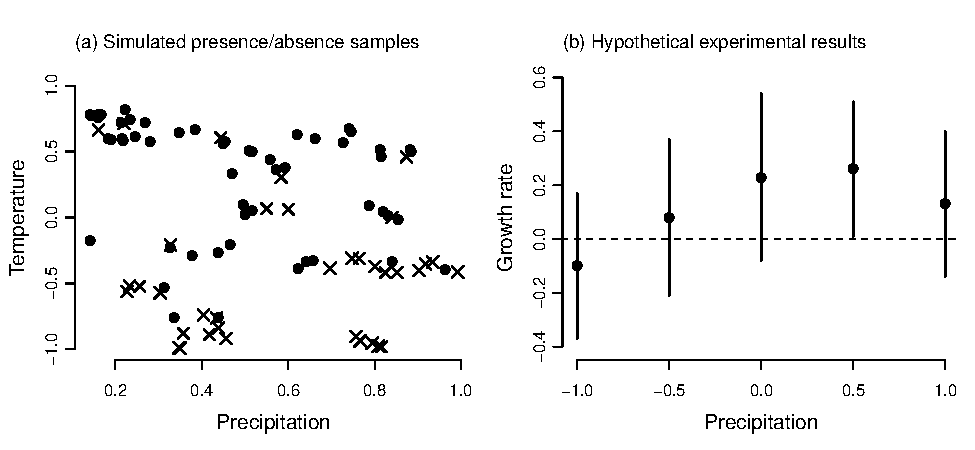
\includegraphics{ex1_sampling.pdf}
	\caption{}
	\label{fig:ex1_sampling}
\end{figure}


%==================
% FIGURE 3
\newpage
\begin{figure}[h!]
	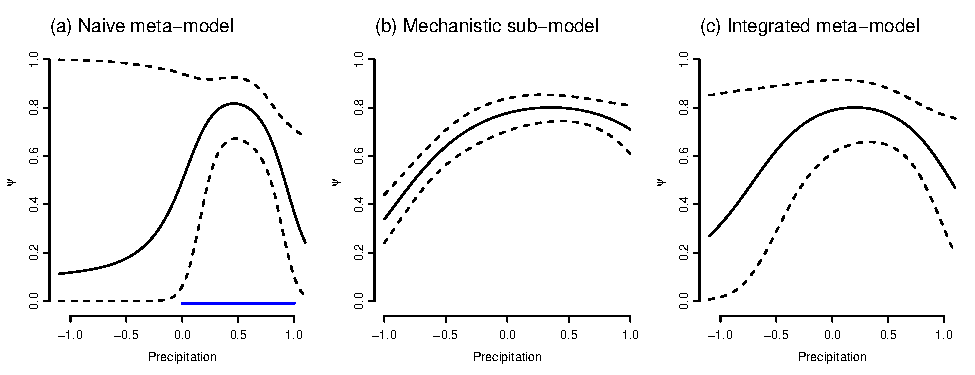
\includegraphics{ex1_precip.pdf}
	\caption{}
	\label{fig:ex1_precip}
\end{figure}


%==================
% FIGURE 4
\newpage
\begin{figure}[h!]
	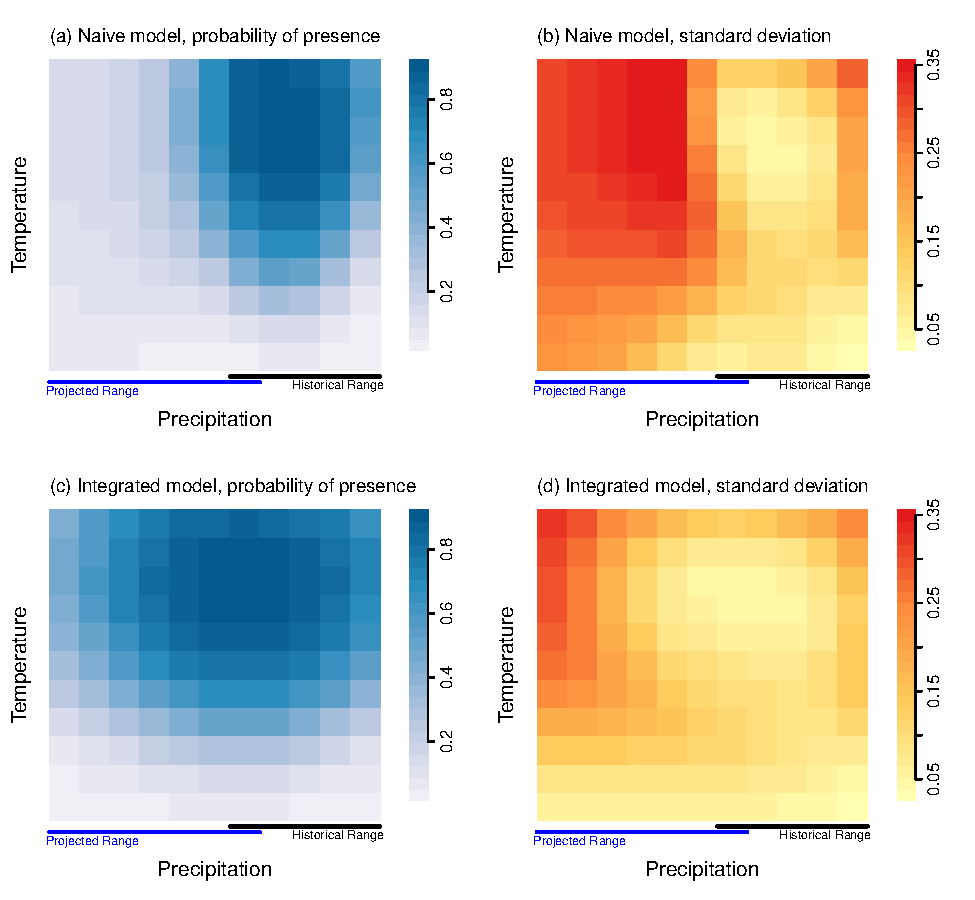
\includegraphics[width=5.25in]{ex1_map.pdf}
	\caption{}
	\label{fig:ex1_map}
\end{figure}


%==================
% FIGURE 5
\newpage
\begin{figure}[h!]
	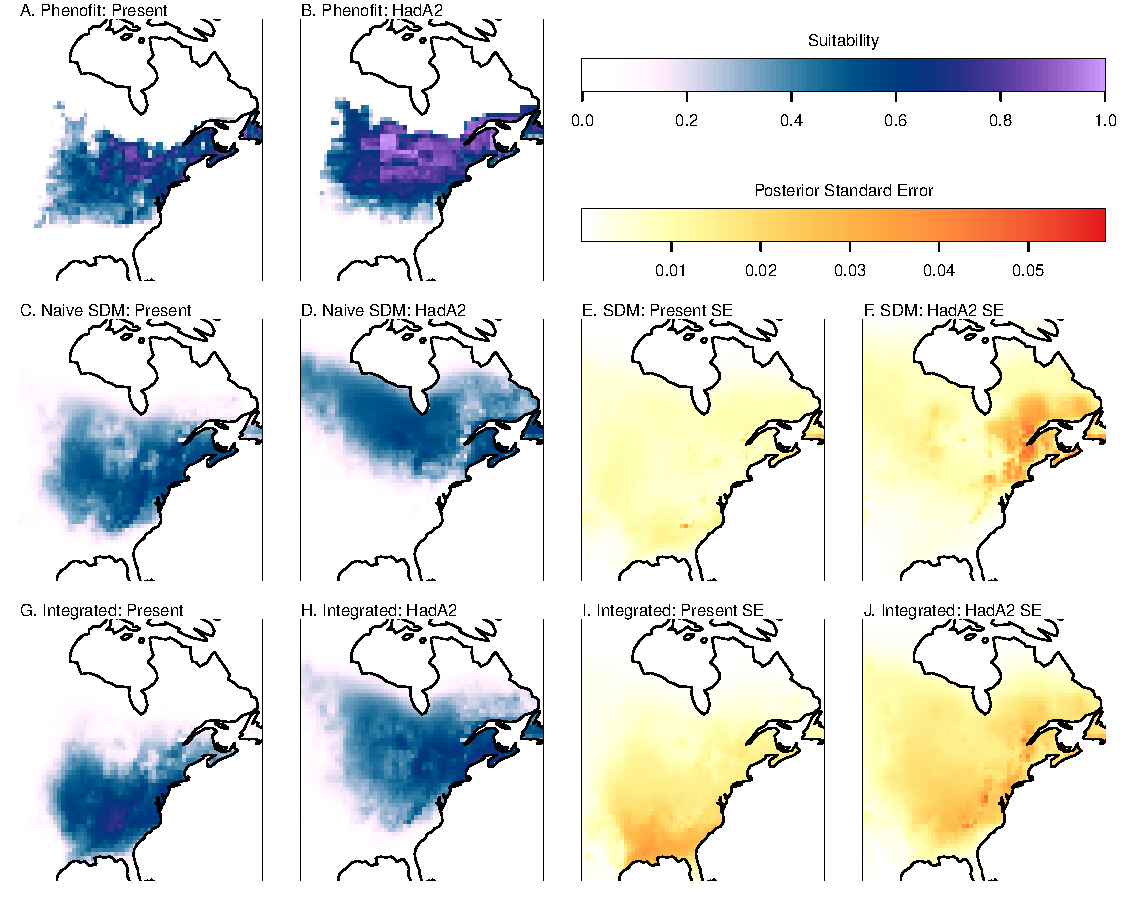
\includegraphics[width=6in]{ex2.pdf}
	\caption{}
	\label{fig:ex2}
\end{figure}


%==================
% FIGURE 6
\newpage
\begin{figure}[h!]
	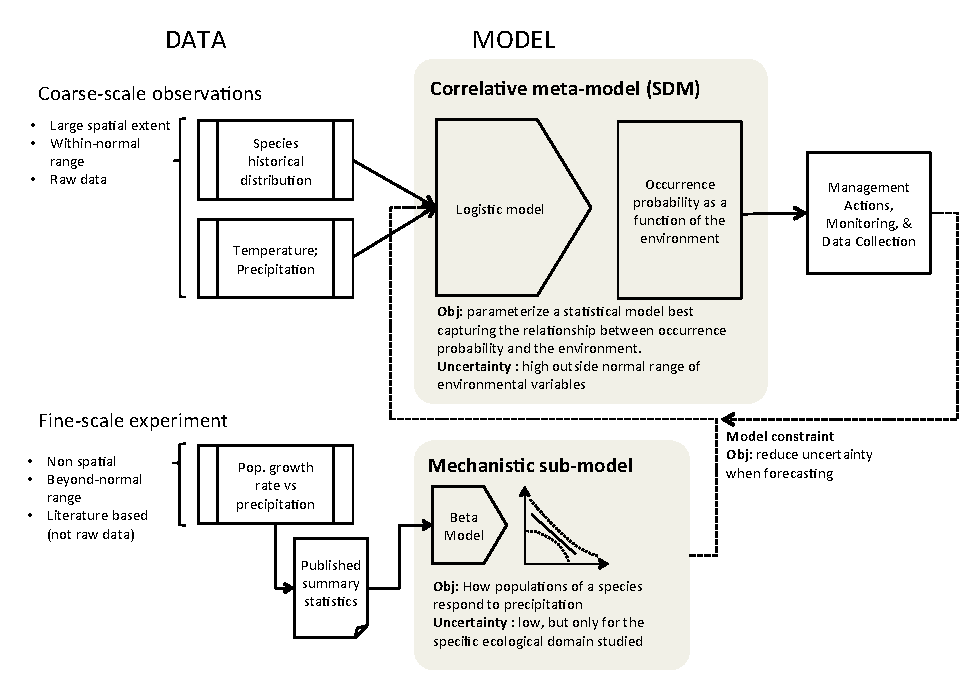
\includegraphics{management.pdf}
	\caption{}
	\label{fig:management}
\end{figure}


%% ----------------------------------
%
%     TEXT BOX
%
%% ----------------------------------

%TC:break box 1

\newpage
\linenumbers
\section*{Box 1: Model description}
% Boxes are limited to 750 words
We begin with a simple correlative model (i.e. calibrated with data provided at the same ecological scale as predictions), characterized in a Bayesian framework to allow further integration. 
We refer to this model (with associated parameters) as the metamodel, \(\theta_M\), and it is parameterized with information on the species' presence, \(X_M\), along with associated covariates (e.g., climate, presence/absence of interacting species, etc.), collectively referred to as \(D_M\). 
The naive (i.e., not integrated with information from sub-models) probability that a species is present, \(\psi_N\), is a deterministic function of the metamodel and its covariates::
%-----
\begin{equation}
\label{eq:sdm1}
	\psi_N = f(\theta_M, D_M)
\end{equation}
%-----
The goal of model fitting is to estimate the posterior probability distribution for the parameters of \(\theta_M\), given the observations (\(X_M\)) and covariates (\(D_M\)):
%-----
\begin{equation}
\label{eq:sdm2}
	p( \theta_M \mid X_M, D_M)
\end{equation}
%-----

Using Bayes' theorem, we find the posterior probability of \(\theta_M\) as follows:
%-----
\begin{equation}
\label{eq:sdm3}
	p( \theta_M \mid X_M, D_M ) = \frac{ p( X_M \mid \theta_M, D_M ) p( \theta_M ) } { p(X_M, D_M) }
\end{equation}
%-----
where \(p( X_M \mid \theta_M, D_M )\) is referred to as the likelihood of the observations, \(p(\theta_M )\) is the prior probability of the model, and \(p(X_M, D_M)\) is the normalization constant.
The normalization constant involves computing integrals that are often impossible to solve analytically. 
In practice, simulation techniques such as \ac{MCMC} can be used to sample directly from the posterior distribution, making such computations unnecessary.
Thus, we use the proportional form of Bayes' Theorem:
%-----
\begin{equation}
\label{eq:sdm4}
	p( \theta_M \mid X_M, D_M ) \propto p( X_M \mid \theta_M, D_M ) p( \theta_M ) 
\end{equation}
%-----

The role of the metamodel is to integrate data at the same ecological scale of predictions.
Additional sub-models require outputs that should be comparable to this given ecological scale (e.g. constraining presence or absence on the landscape).
Formally, we will add an additional model, \(\theta_S\), that is based on a different set of hypotheses and that makes predictions \((\psi_S)\) based on an additional dataset \((X_S, D_S)\):
%-----
\begin{equation}
\label{eq:model2-1}
	\psi_S = g(\theta_S, X_S, D_S)
\end{equation}
%-----

For integration to be successful, it must be possible to compute the likelihood of this prediction given the metamodel, \(p \left( \psi_S \mid \theta_M \right) = p \left(\theta_S \mid \theta_M, X_S, D_S \right)\); the function \(g\) serves to transform the parameters of the sub-model to the scale of the metamodel. Thus, we refer to $g$ as the \emph{scaling function}. 
In many cases, computing this likelihood will be challenging.
The simplest case is when the parameters of \(\theta_S\) are directly comparable to those in \(\theta_M\) (see Example 1), or when the scaling is performed directly within the sub-model (see Example 2), but other solutions are possible.
This new likelihood, which integrates the information from the second model into the first, can be treated as new ``data'' to evaluate the parameters of \(\theta_M\).
We simply use the posterior distribution of $\theta_M$ from the previous step (Eq. \ref{eq:sdm4}) as the new prior probability of $\theta_M$, and evaluate the posterior probability of $\theta_M$ in light of the new data (i.e., information from the submodel \(\theta_S\)) and the prior knowledge, as before:

%-----
\begin{equation}
\label{eq:integrated2}
	\overbrace{p( \theta_M \mid X_M, D_M, \theta_S, X_S, D_S )}^\text{integrated posterior}
	\propto 
	\overbrace{p( \theta_S \mid \theta_M, X_S, D_S )}^\text{likelihood}
	\overbrace{p( X_M \mid D_M, \theta_M ) P( \theta_M )}^{\text{prior for } \theta_M}
	\overbrace{p(\theta_S)}^{\text{prior for } \theta_S}
\end{equation}
%-----

This procedure may be repeated 
\wt{replace by applied or used. 
Here looks like you have to repeat this to add a new model for instance. }
for an arbitrary number of models (limited only by available data and computational power). 
The models may be implemented simultaneously, when multiple datasets are available and can be evaluated under different underlying models, or they may be run sequentially, updating the posterior distribution of $\theta_M$ as new information becomes available. 
Note that $\theta_S$ itself need not be implemented in a Bayesian framework and the output need not be identical in form to the output of \(\theta_M\); it is enough to produce an output that can be evaluated as a likelihood under the first model and to have some assessment of the confidence in the parameter estimates of $\theta_S$ to use as a prior.

%---------------------------------------------
%---------------------------------------------


\end{document}